\section{Brake Force Acquisition Channel}\label{sec:brake-pressure-acquisition-channel}

\subsection{Load Cell Signal}\label{ssec:load-cell-signal}

	Load cells have very low output levels, usually from 2 to 3mV for each volt applied at the bridge, and therefore an amplification stage is fundamental. It is not necessary to know the nature of the strain gauges when a load cell is being calibrated since generally the manufacturers provide a calibration curve based on the signals $V_{O}$ and $V_{EX}$ of the Figure \ref{fig:wheatstone}, it is worth noting that these signals can not have the same reference, otherwise it will not be possible to excite the wheatstone bridge correctly.
	\par
	The most common way to amplify the signal of a load cell is using a instrumentation amplifier. Although it is a widely used configuration, assembling this amplifier using three different operational amplifiers and seven resistors as in Figure \ref{fig:instrumentation-amplifier} may make it inaccurate due to manufacturing imperfections of the components. Another factor that greatly influences the output signal of a load cell is the excitation voltage of its wheatstone bridge, if it varies too much the output will vary greatly as well, which will hamper its calibration.

\subsection{Load Cell Signal Conditioning}\label{ssec:load-cell-signal-conditioning}
		
	In order to solve these two problems there is a solution widely used in the market which is the \textit{INA125} from Texas Instruments \cite{ina125}, this IC is an integrated single supply instrumentation amplifier with precision voltage reference. Other good feature of this amplifier is that as it has a great CMRR (\textit{Common-Mode Rejection Ratio} check Section \ref{itm:opamp-cmrr}) of 100dB, making it very much suitable for conditioning differential pair signals (such as the one from the Load Cell as Subsection \ref{ssec:brakeForceMeasurement} mentions), more information of CMRR in Subsection \ref{sssec:important-features-to-consider-in-a-amplifier}. The only external component needed is a resistor $R_{G}$, as shown in Figure \ref{fig:ina125-functional-block}. This resistor will determine the gain (G) for the amplification according to the Equation \ref{eqn:ina125-g}.
	

	\begin{figure}[htbp]
		\centering
		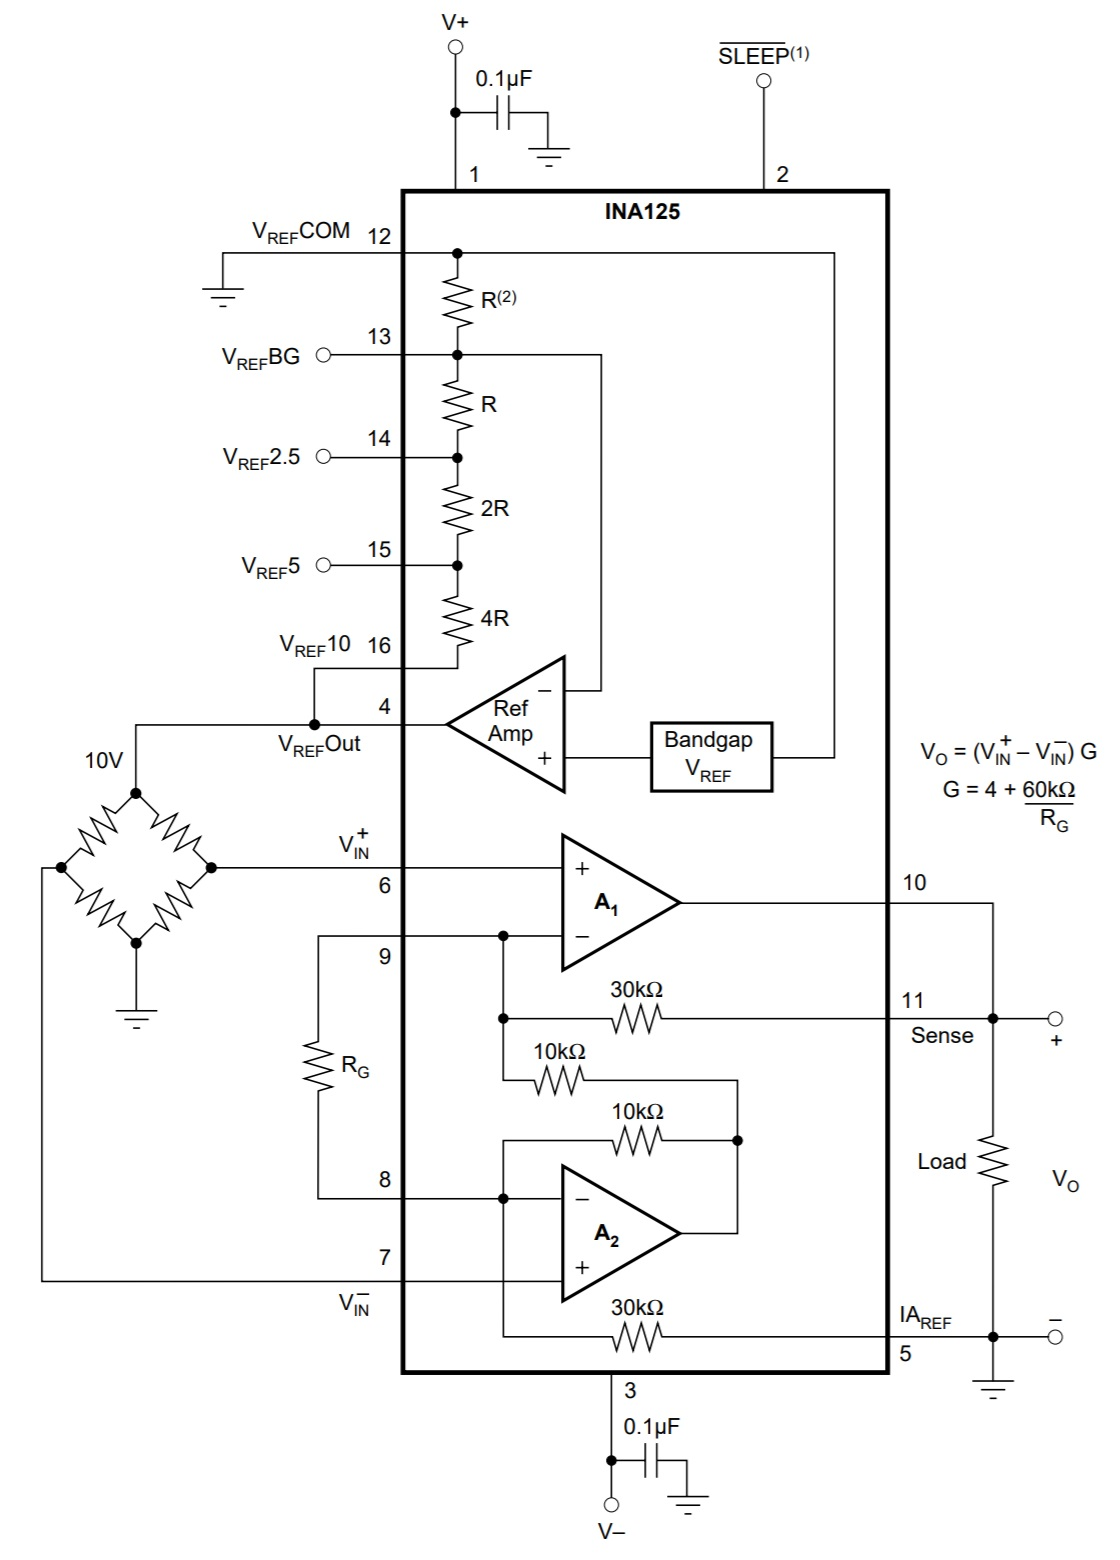
\includegraphics[width=.6\textwidth]{figuras/fig-ina125-functional-block}
		\caption{INA125 Schematic \cite{ina125}}
		\label{fig:ina125-functional-block}
	\end{figure}

	\begin{equation}\label{eqn:ina125-g}
		R_{G}=\frac{60k\Omega}{G - 4}
	\end{equation}

	Taking into account the sensitivity of 2mV/V, this means that if the cell is excited with 2V5, its output will vary from 0 to 5mV.
	\par
	Since the analog input of the chosen microcontroller \textit{(Atmega32U4)} is 0 to 5V, we may to amplify the cell output signal by a factor of 500 in order to use the most number of bits from de MCU's ADC. Using Equation \ref{eqn:ina125-g}, to obtain a gain of amplification ratio of the ideal $R_{G}$ would be 121$\Omega$. This resistor will cause the IC output to range from about 0V to 5V (0 to 2.5V for contraction and 2.5V to 5V for tension), using 100\% of the resolution of the microcontroller input. 
	\par
	Figure \ref{fig:cic-cell} shows the schematic of the load cell conditioning circuit with the INA125.

	\begin{figure}[htbp]
		\centering
		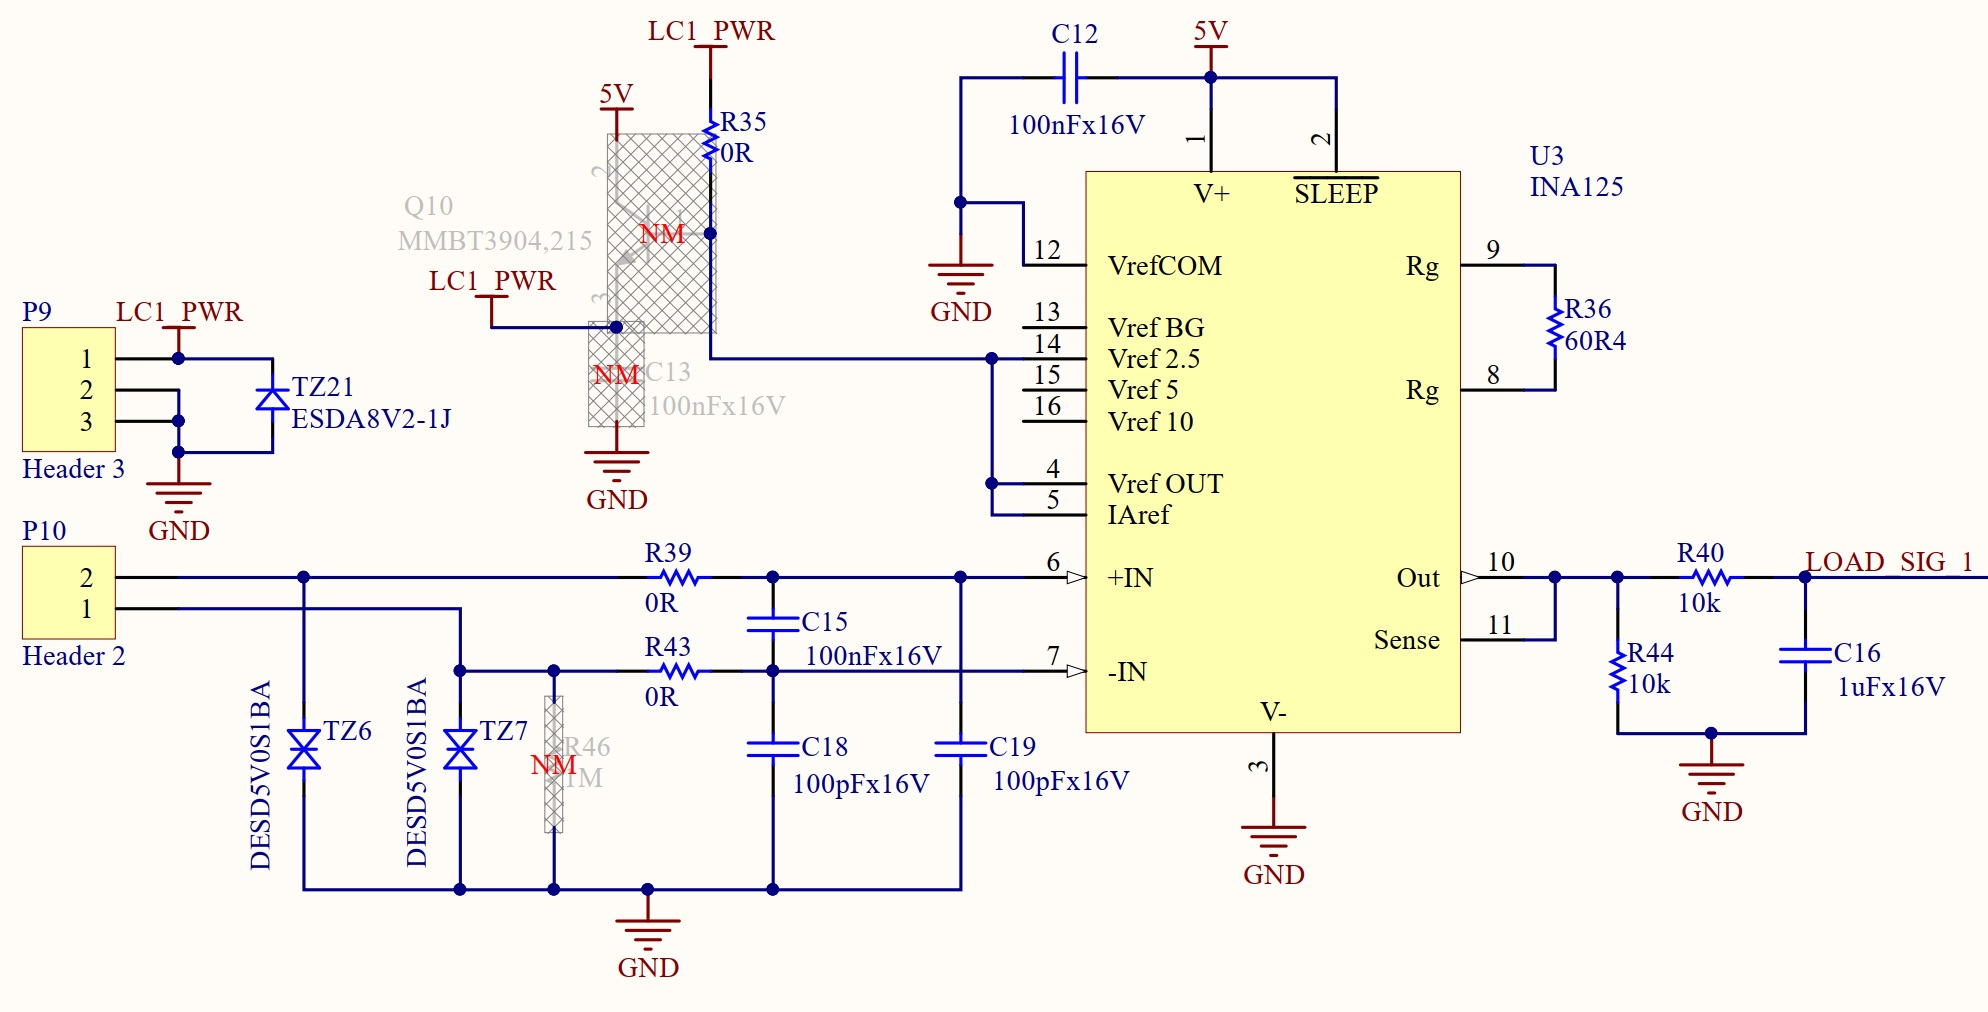
\includegraphics[width=1\textwidth]{figuras/fig-cic-cell}
		\caption{Conditioning Circuit for the Load Cell}
		\label{fig:cic-cell}
	\end{figure}

	The main components of this circut are
	\begin{itemize}
		\item\textit{TVS Diodes:} INA125 only has overvoltage protection and not ESD protection, so the TVS Diodes were add to enhance the ESD protection.
		\item\textit{Capacitors C18 and C19:} Bypass capacitors for the signal lines.
		\item\textit{C15:} A capacitor to filter noise between both lines.
		\item\textit{R39 and R43:} Jumpers that can be replaced by resistors in case a RFI filter is meant to be implemented using C24, C26 and C27.
		\item\textit{R36:} The gain resistor.
		\item\textit{R44, R40 and C16:} R44 is used to set the impedance from the load cell signal. R40 and C16 are used to form a LPF with a cutoff frequency of 15.91Hz to filter any remaining noise from the load cell signal.
	\end{itemize}

\subsection{Load Cell Sensor Detection}\label{ssec:load-cell-sensor-detection}
	As was explained in Subsection \ref{ssec:load-cell-signal-conditioning}, the circuit will saturate the output to the supply voltage when the load cell sensor is disconnected. The circuit to detect this voltage saturation is exact the same from the one used previously on the thermocouple circuit, the circuit schematic and functional explanation can be found in Subsection \ref{ssec:thermocouple-sensor-detection}.